\section{Ferramentas Utilizadas}

\subsection{Linguagens e \textit{Frameworks}}

O aplicativo Guimifiu está sendo desenvolvido utilizando o \textit{framework} Ionic 2, que por sua vez utiliza TypeScript como linguagem de programação. O TypeScript é uma linguagem que facilita o desenvolvimento em JavaScript em larga escala. É uma linguagem fortemente tipada, e que facilita a aplicação de orientação a objetos em aplicações JavaScript. O TypeScript é compilado e transformado em JavaScript \cite{typescript}. O Ionic 2 é um \textit{framework} livre criado pela \textit{Drifty Co.} em 2012 que empacota o Cordova e o TypeScript para utilizar funções nativas dos aparelhos móveis e criar aplicativos multi-plataforma a partir de um único código \cite{ionic-2}.

Em conjunto com o desenvolvimento do aplicativo, está sendo desenvolvido uma API RESTful utilizando a linguagem de programação Ruby com o \textit{framework} Ruby on Rails. Criado em 1995, o Ruby é uma linguagem de tipagem dinâmica \textit{open source} que foi criada como sendo uma junção das melhores partes das linguagens Perl, Smalltak, Eiffel, Ada e Lisp. O Ruby permite \textit{multithreading} independente se o sistema operacional suporta ou não \cite{ruby-wow}. O Ruby on Rails é um \textit{framework} criado em 2004 para desenvolvimento de aplicações \textit{web} que faz com que o programador use o paradigma de convenção sobre configuração \cite{rails}. Vários softwares são desenvolvidos em Ruby on Rails como o GitHub, Shopify, Hulu e Twitch. A representação dos dados da API são em JSON.

\subsection{Testes}

Para a aplicação \textit{mobile}, foram utilizados os \textit{frameworks open source} Jasmine para escrever os testes e o Karma para rodar a suíte. O Karma é um ambiente de teste para JavaScript que os desenvolvedores conseguem \textit{feedbacks} rápidos do código que estão desenvolvendo \cite{karma}. O Jasmine é um \textit{framework} que utiliza conceitos de \textit{behavior-driven development} para escrever testes \cite{jasmine}. O CodeCov foi utilizado para adquirir a cobertura de código dos testes.

Para a API, foi utilizado o RSpec, que é uma ferramenta para escrever e executar a suíte de testes \cite{rspec} e o Coveralls que adquire a cobertura de código dos testes \cite{coveralls}.

\subsection{Métricas de Código-fonte}
Para as métricas de código-fonte da aplicação \textit{mobile}, foi utilizado o TSLint, que checa código TypeScript em questões de manutenabilidade, leitura e erros funcionais \cite{tslint}.

No código-fonte da API foi utilizado o CodeClimate, uma ferramenta que baixa o código do Github e checa em seus servidores a complexidade do código, duplicação, estilo e segurança \cite{codeclimate}. O CodeClimate utiliza as seguintes para gerar o relatório final:
\begin{itemize}
    \item \textbf{Reek:} para verificação de \textit{code smells}, que são sintomas no código-fonte que podem gerar problemas;
    \item \textbf{Flog:} para a verificação da complexidade do código Ruby;
    \item \textbf{Rubocop:} que verifica estilo e qualidade do código;
    \item \textbf{Brakeman:} para uma verificação estática de segurança do código.
\end{itemize}

Além disso, é também uma ferramenta própria do CodeClimate para checagem de duplicações de código.

O Rubocop foi utilizado também fora do CodeClimate para medir a complexidade do código. Além de complexidade, o Rubocop possui diversas outras ferramentas embutidas que verificam outros aspectos baseados no guia de estilo do Ruby mantido pela comunidade \cite{rubocop}. Os padrões mínimos ou máximos dessas outras ferramentas serão analisadas com o desenvolvimento do projeto.

\subsection{Integração e Entrega Contínua}

O TravisCI é uma ferramenta grátis para projetos \textit{open source} que faz a integração contínua de projetos em várias linguagens. As \textit{builds} são feitas imediatamente após os \textit{pushes} na ferramenta de controle de versão e, através de um script criado pelo usuário, o Travis configura e roda a suíte de testes do \textit{commit}. Além disso, o Travis também pode fazer \textit{deploys} no Heroku caso a \textit{build} esteja passando \cite{travis-ci}.

O Heroku é uma plataforma que permite criar, entregar, monitorar e escalar aplicativos. Comumente utilizado para o \textit{deploy} de aplicações web, o Heroku também serve para hospedar serviços na nuvem, facilitando a arquitetura de aplicativo-API \cite{heroku}.

O Fastlane é uma ferramenta \textit{open source} para automatizar a entrega contínua de aplicativos iOS e Android. Ele conecta diretamente com a App Store e a Play Store para fazer \textit{deploys} das versões do aplicativo, inclusive versões beta exclusivas para testes \cite{fastlane}.

\subsection{Prototipação}

Após a finalização do \textit{Crazy Eights}, foi escolhido as melhores telas para serem levadas como base da construcação do aplicativo. Com os requisitos validados, foram desenhados protótipos de baixa fidelidade para as histórias de usuários que seriam desenvolvidas. Sendo assim, a prototipação fez o uso de duas ferramentas:

\begin{itemize}
    \setlength\itemsep{0em}
    \item \textbf{Marvelapp:} utilizado para simular o fluxo das telas geradas pelo \textit{Crazy Eights}, onde é possível tirar fotos dos protótipos desenhados e criar transições nas telas desenhadas de forma a mostrar o fluxo da aplicação, que pode ser tanto web quando para Android e iOS \cite{marvelapp};
    \item \textbf{NinjaMock:} utilizado para a prototipação de baixa fidelidade das histórias de usuário. É uma ferramenta de criação de \textit{wireframe designs} para plataformas móveis e web \cite{ninjamock}.
\end{itemize}

A Figura \ref{img:prototipo_de_papel_tela_de_login} mostra o protótipo de papel da tela de login da aplicação. O login pode ser feito via Facebook, Google ou criando uma conta local.
\begin{figure}[H]
    \centering
    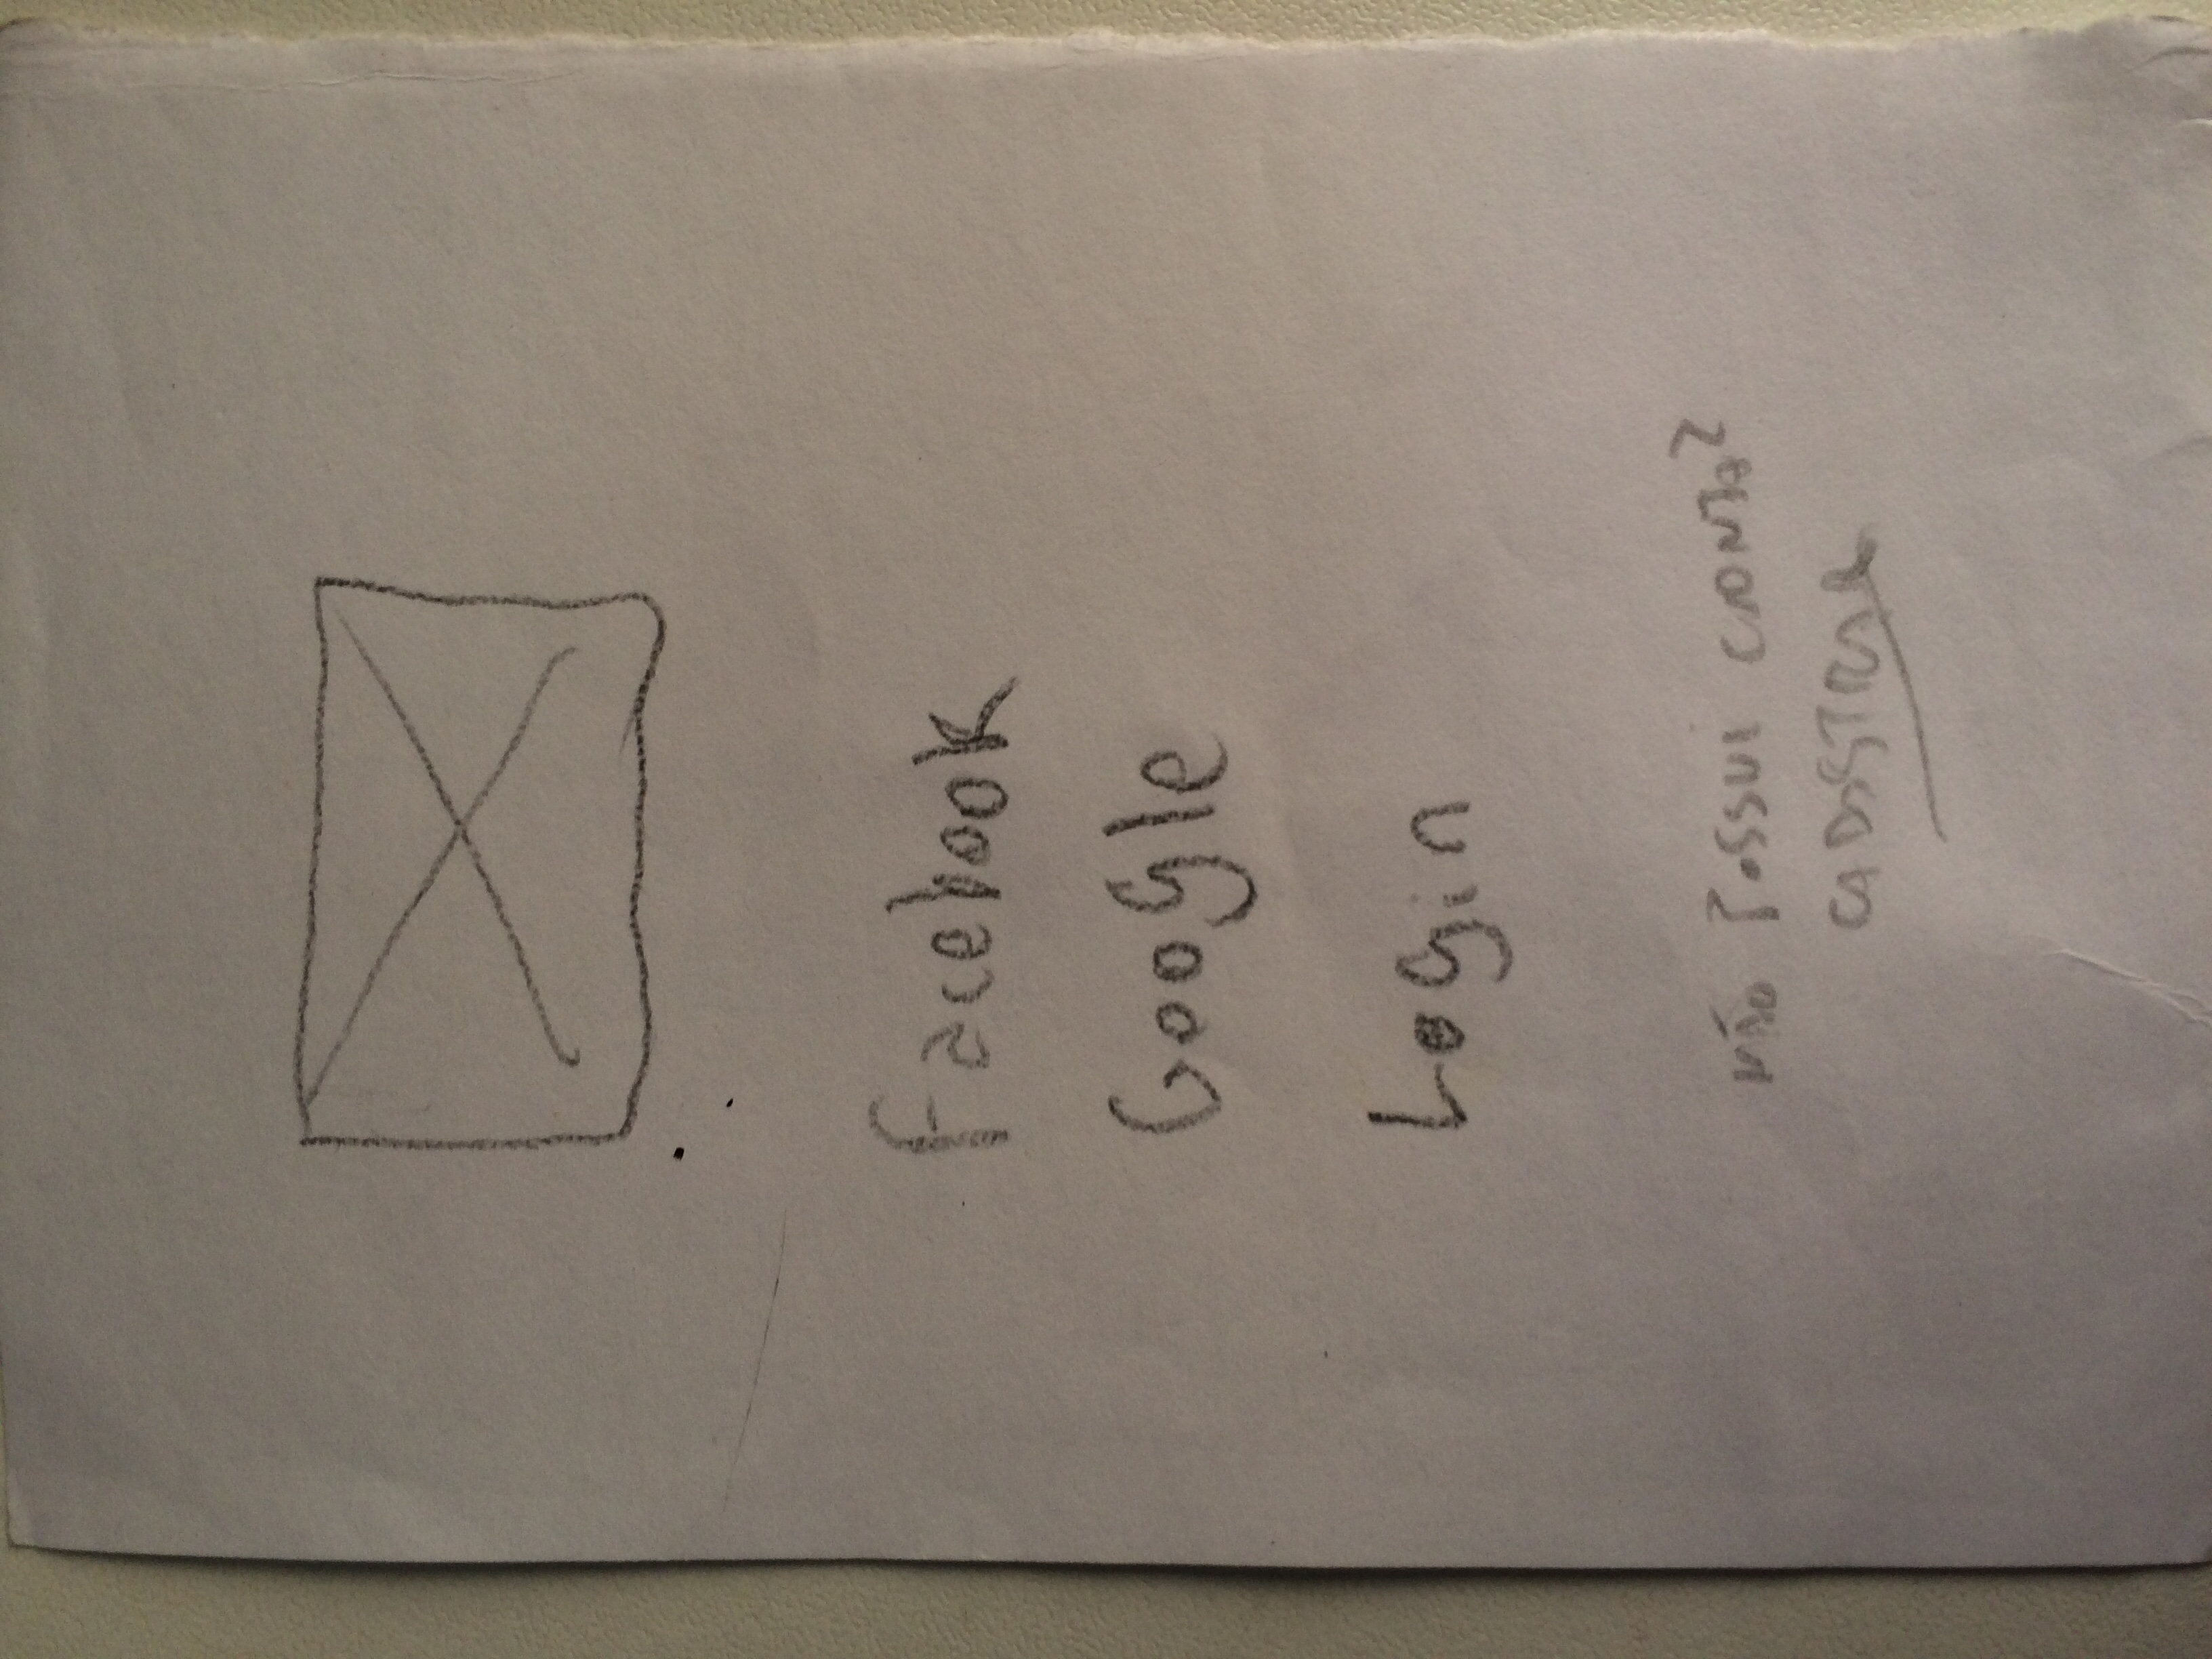
\includegraphics[scale=0.05, angle=-90]{figuras/prototipo_papel_login.jpg}
    \caption[Protótipo de papel da tela de login]{Protótipo de papel da tela de login. Fonte: autores}
    \label{img:prototipo_de_papel_tela_de_login}
\end{figure}
\pagebreak

A Figura \ref{img:prototipo_de_papel_tela_incial} mostra o protótipo de papel da tela inicial da aplicação. Um mapa será mostrado com algumas informações do usuário.
\begin{figure}[H]
    \centering
    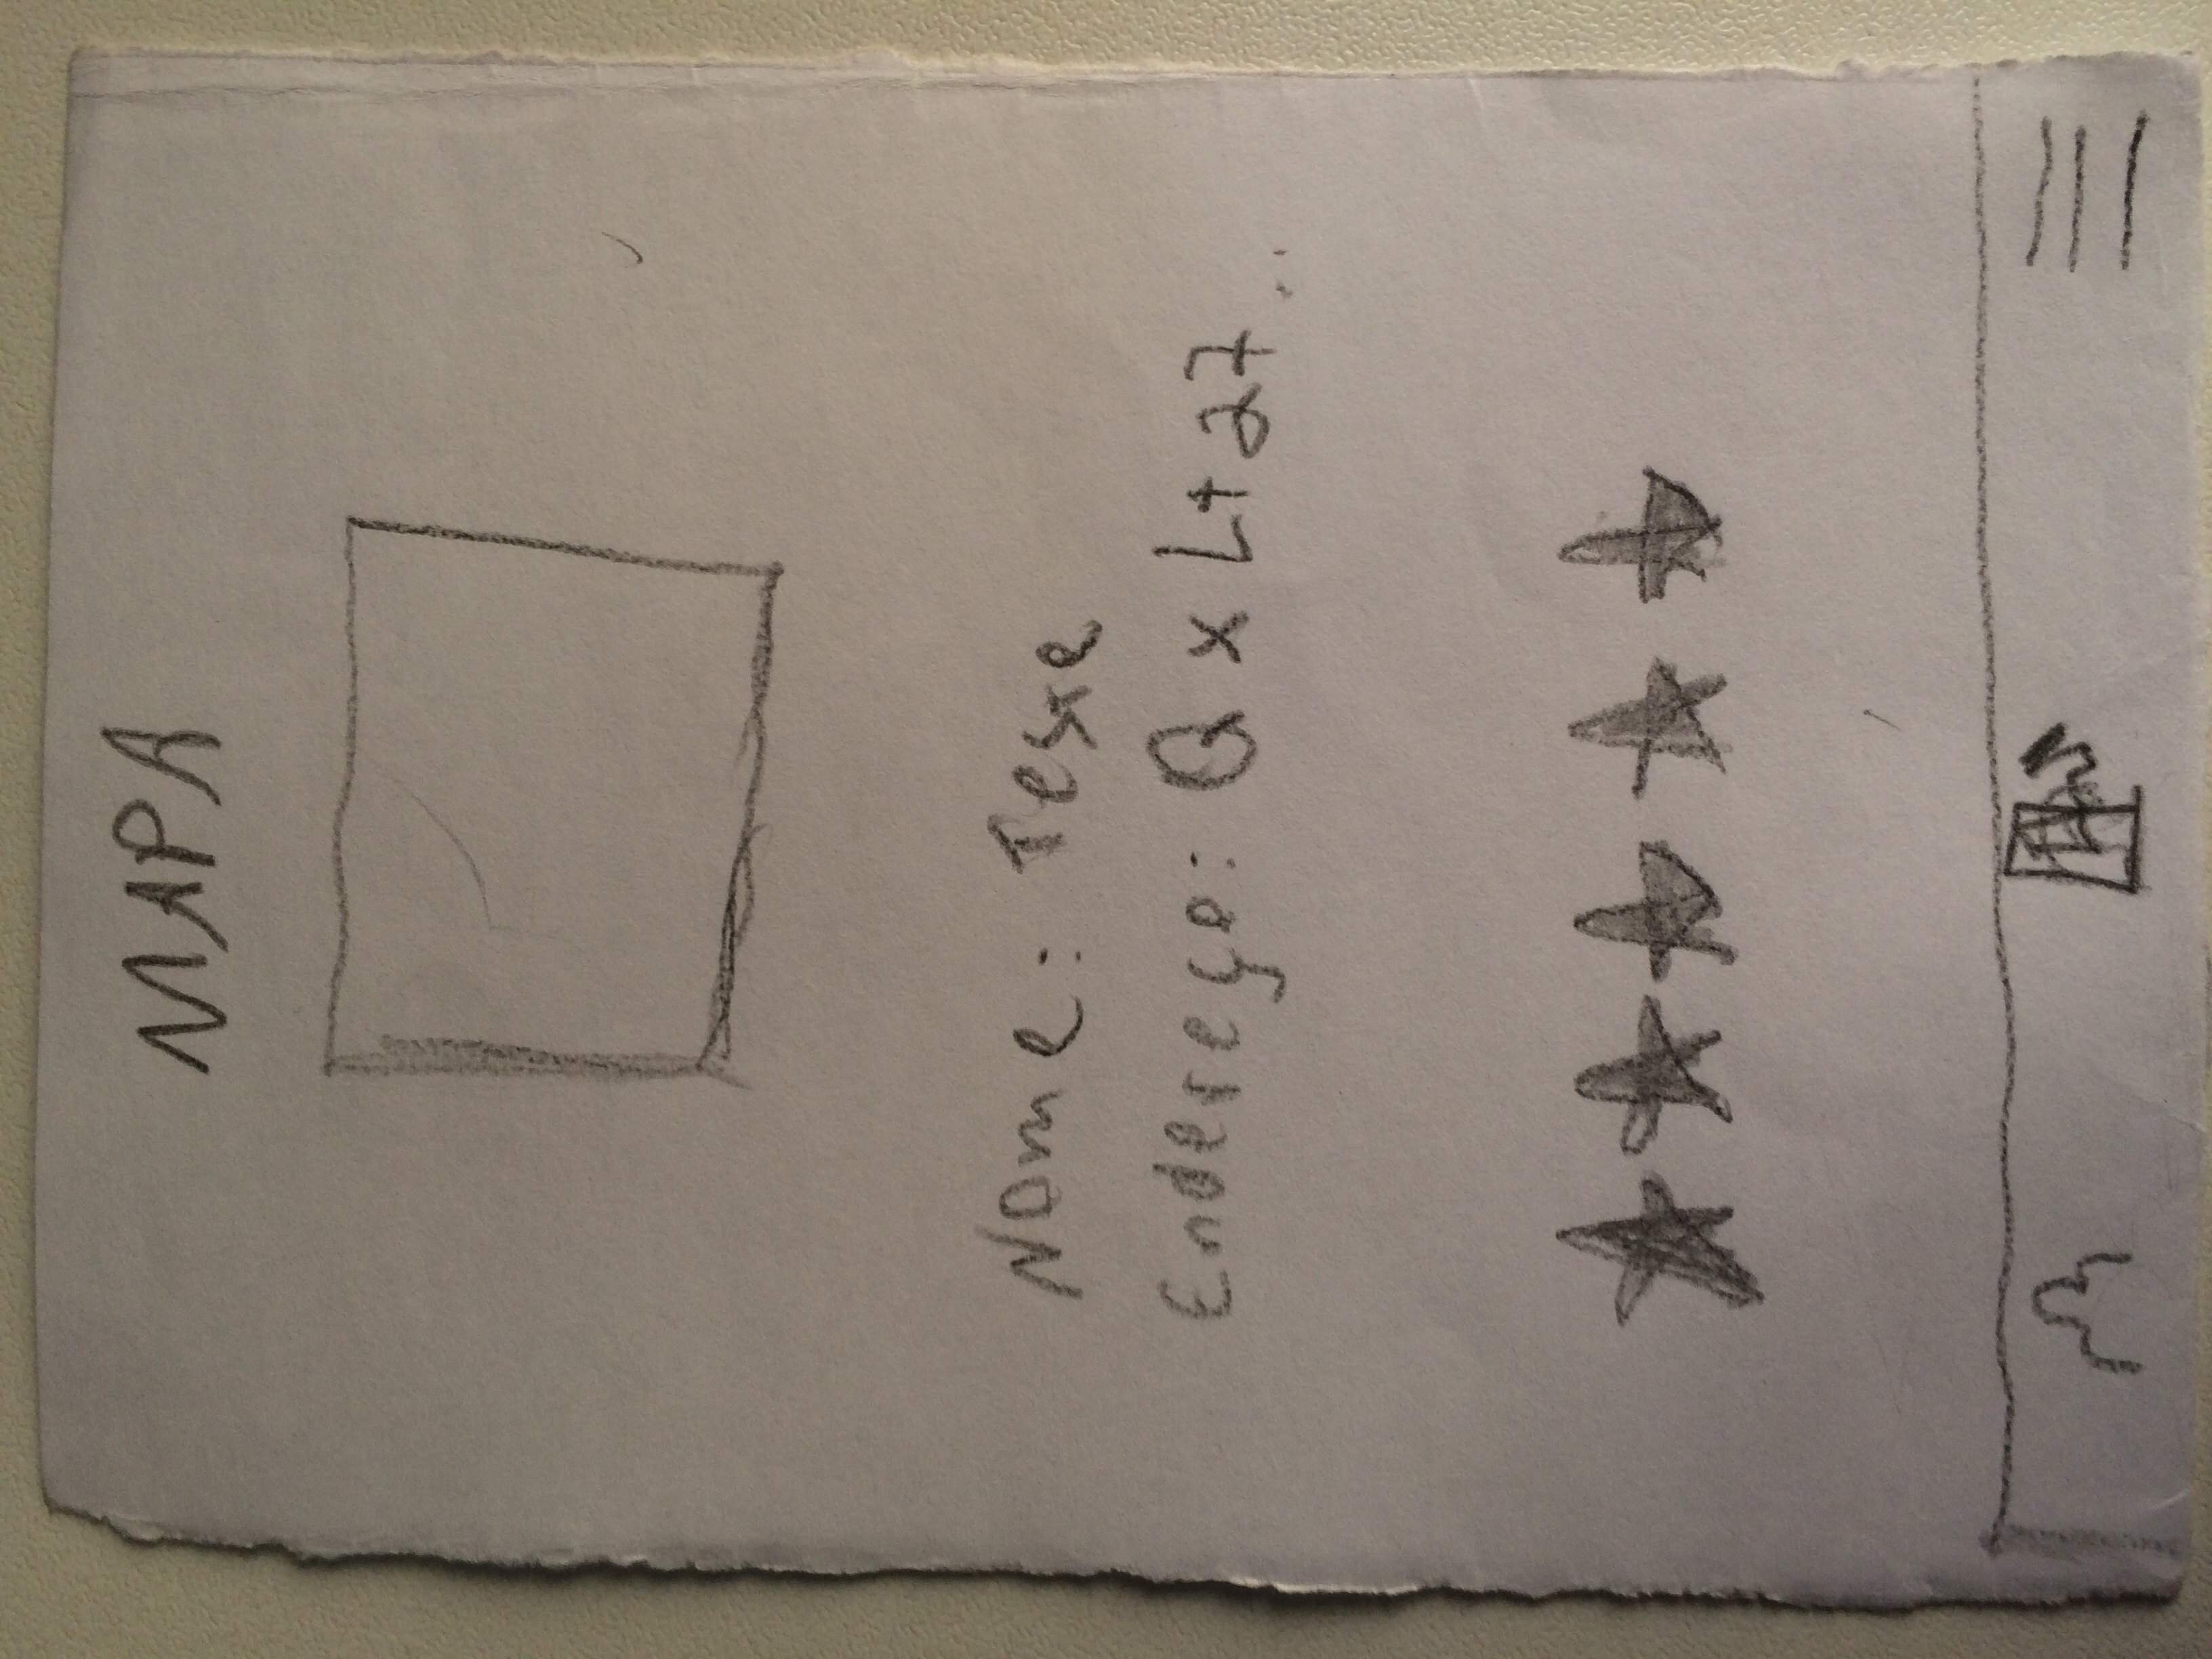
\includegraphics[scale=0.05, angle=-90]{figuras/prototipo_papel_inicial.jpg}
    \caption[Protótipo de papel da tela inicial]{Protótipo de papel da tela inicial. Fonte: autores}
    \label{img:prototipo_de_papel_tela_incial}
\end{figure}

A Figura \ref{img:prototipo_de_papel_menu_lateral} mostra o protótipo de papel do menu lateral da aplicação.
\begin{figure}[H]
    \centering
    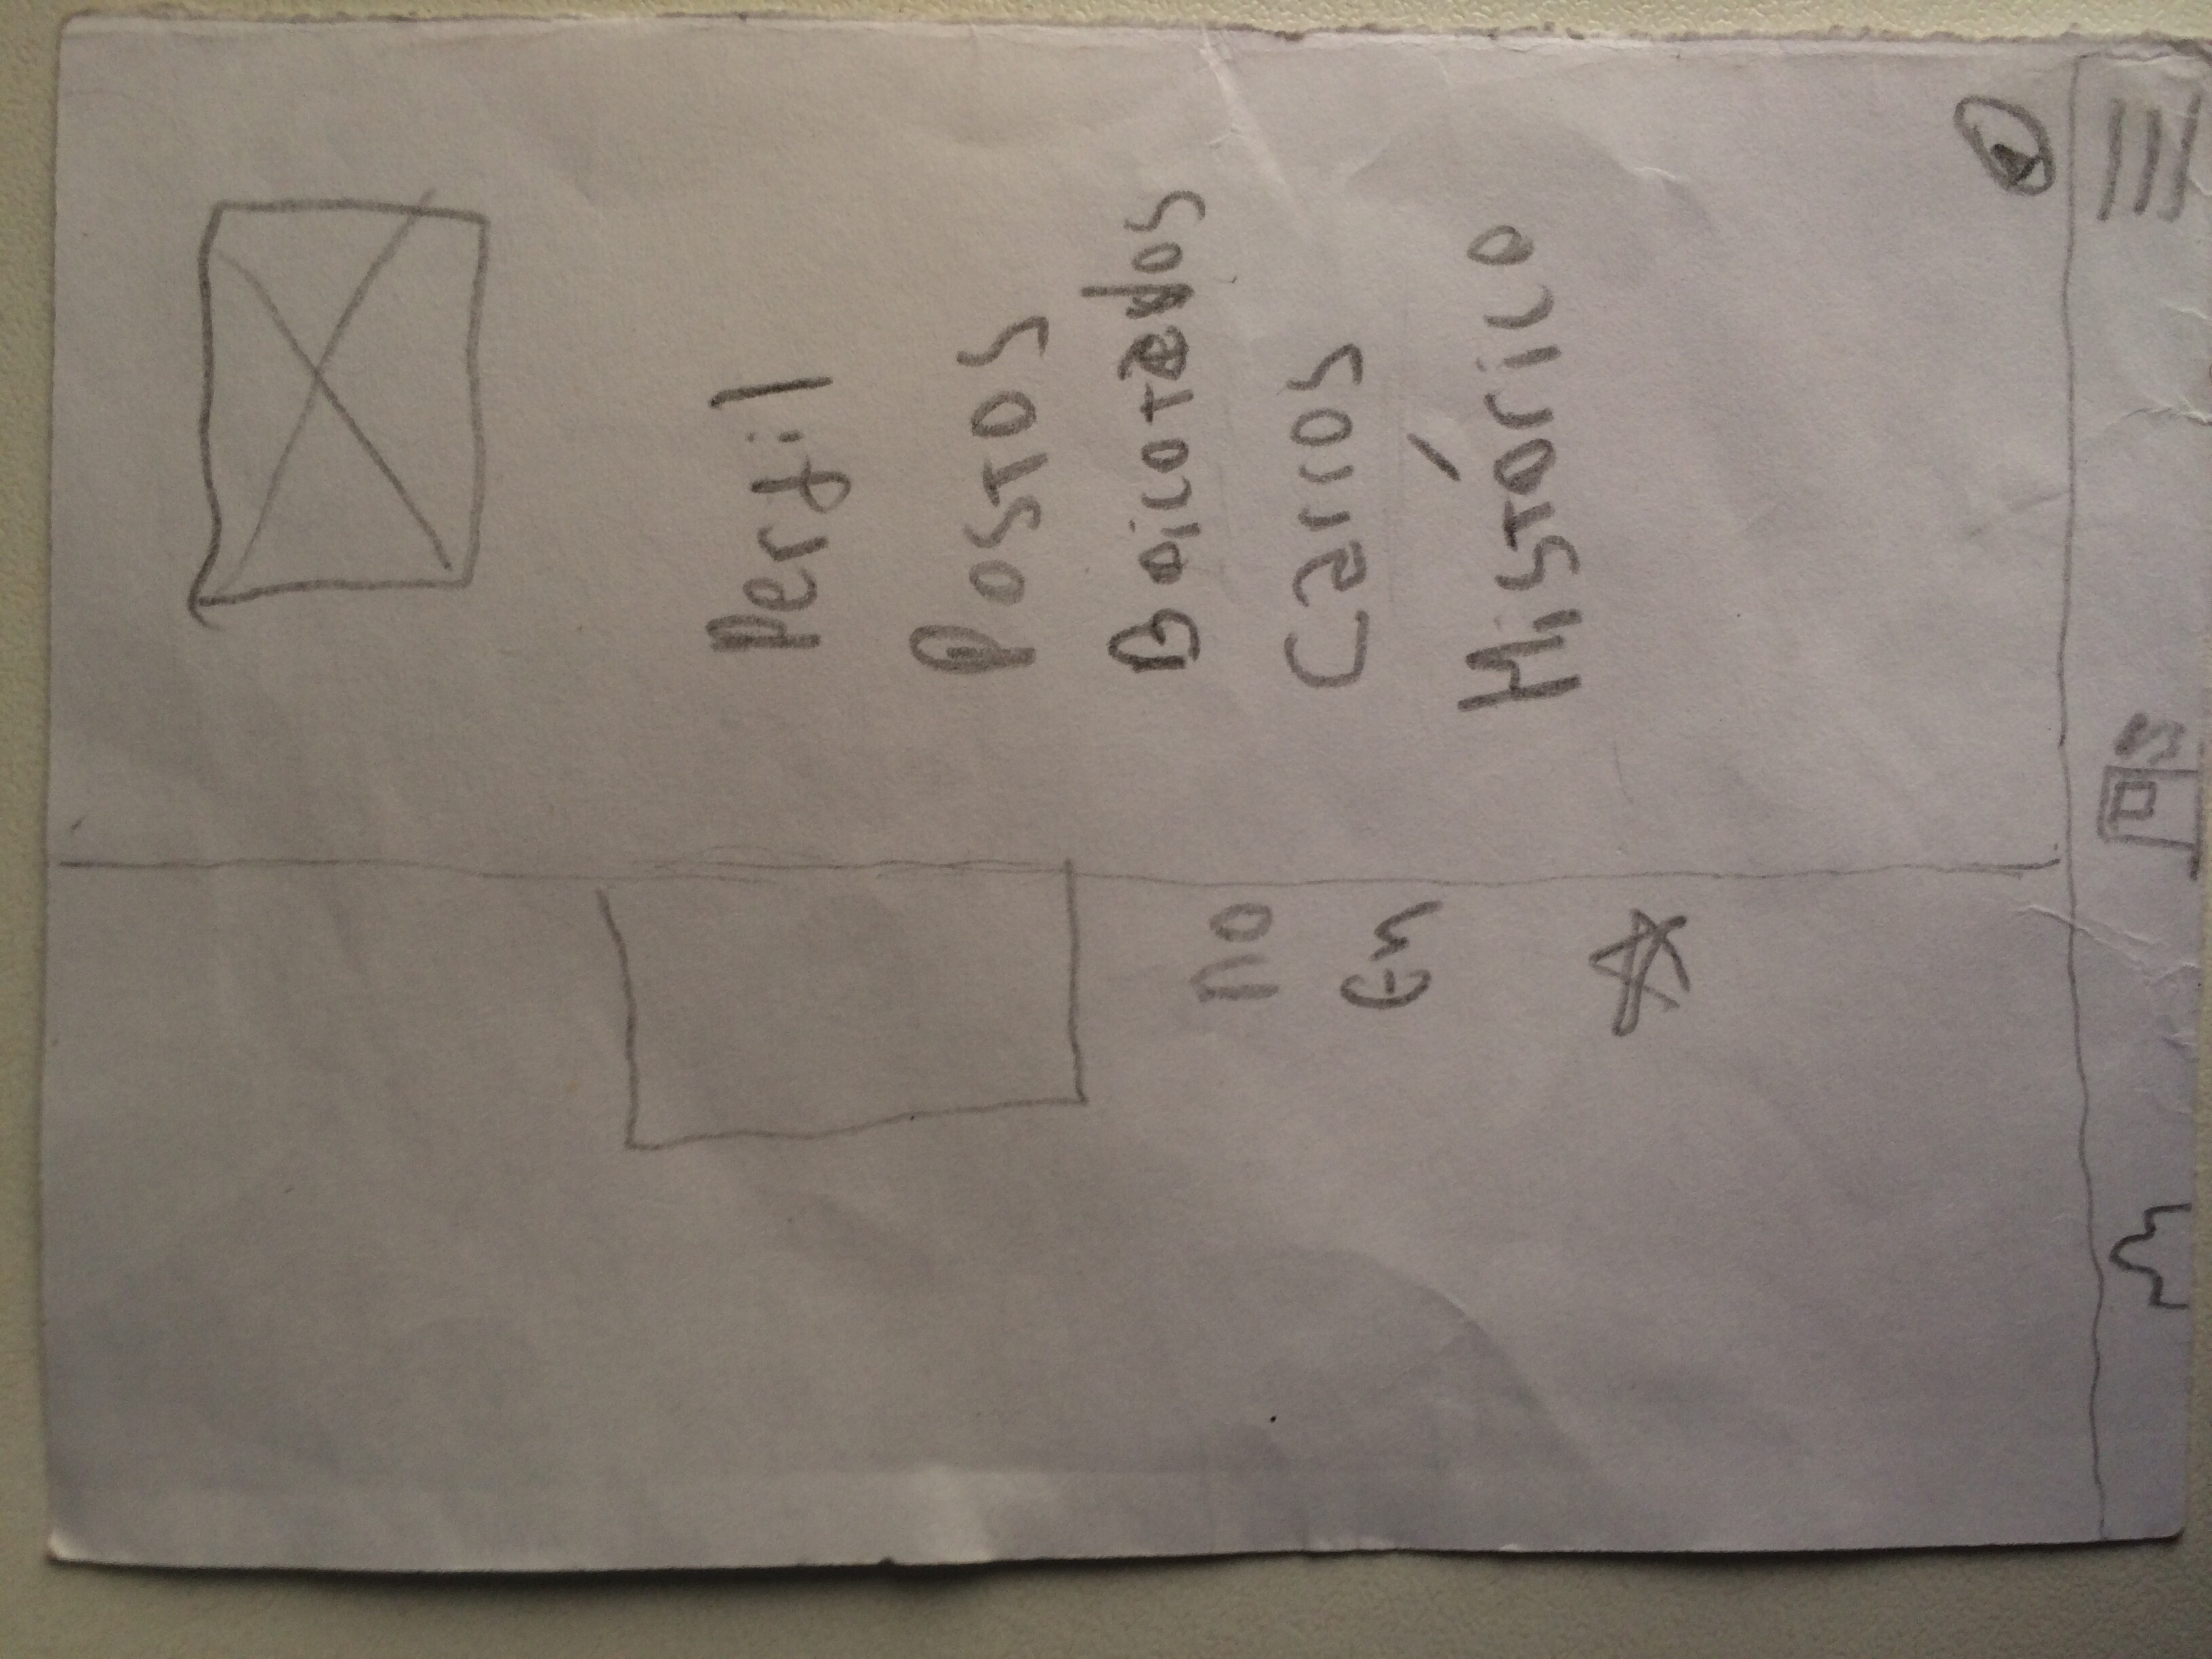
\includegraphics[scale=0.05, angle=-90]{figuras/prototipo_papel_menu.jpg}
    \caption[Protótipo de papel do menu lateral]{Protótipo de papel do menu lateral. Fonte: autores}
    \label{img:prototipo_de_papel_menu_lateral}
\end{figure}

Os demais protótipos se encontram no Apêndice \ref{chap:prototipo}

\subsection{Comunicação}

A comunicação da equipe foi em sua maioria pela ferramenta Slack. O Slack é uma ferramenta de comunicação através de canais de mensagens. O objetivo é que cada canal tenha o seu respectivo assunto para organizar o projeto que podem ser: públicos, ou seja, para todos os membros da equipe; ou privados, ou seja, para apenas uma parte da equipe \cite{slack}. Além disso, é possível integrar outras ferramentas no Slack, para mostrar eventos como \textit{commits} do GitHub, resultados de \textit{builds} do TravisCI, entre outras, assim evitando ter que abrir múltiplas ferramentas para ver os resultados dos trabalhos dos outros. As ferramentas integradas com o Slack foram:

\begin{itemize}
    \item GitHub;
    \item TravisCI;
    \item CodeCov;
    \item Coveralls;
    \item Fastlane;
\end{itemize}

Todas as ferramentas foram integradas em um único canal para facilitar a organização dos eventos durante o desenvolvimento.
